\documentclass{article}
\usepackage{amsmath}
\usepackage[utf8]{inputenc}
\usepackage{graphicx}
\usepackage{verbatim}
\usepackage{float}
\usepackage[makeroom]{cancel}
\usepackage[english]{babel}
\usepackage{textcomp}
\usepackage{gensymb}
\usepackage{color}
\usepackage{subcaption}
\usepackage{caption}
\usepackage{hyperref}
\usepackage{physics}
\usepackage{dsfont}
%\usepackage{amsfonts}
\usepackage{listings}
\usepackage{multicol}
\usepackage{units}

% From Eirik's .tex
\usepackage{epstopdf}
\usepackage{cite}
\usepackage{braket}
\usepackage{url}
\bibliographystyle{plain}

\usepackage{algorithmicx}
\usepackage{algorithm}% http://ctan.org/pkg/algorithms
\usepackage{algpseudocode}% http://ctan.org/pkg/algorithmicx

\usepackage[margin=1cm]{caption}
\usepackage[outer=1.2in,inner=1.2in]{geometry}
% For writing full-size pages
%\usepackage{geometry}
%\geometry{
%  left=5mm,
%  right=5mm,
%  top=5mm,
%  bottom=5mm,
%  heightrounded,
%}

% Finding overfull \hbox
\overfullrule=2cm

\lstset{language=IDL}
 %\lstset{alsolanguage=c++}
\lstset{basicstyle=\ttfamily\small}
 %\lstset{backgroundcolor=\color{white}}
\lstset{frame=single}
\lstset{stringstyle=\ttfamily}
\lstset{keywordstyle=\color{red}\bfseries}
\lstset{commentstyle=\itshape\color{blue}}
\lstset{showspaces=false}
\lstset{showstringspaces=false}
\lstset{showtabs=false}
\lstset{breaklines}
\lstset{aboveskip=20pt,belowskip=20pt}

\lstset{basicstyle=\footnotesize, basewidth=0.5em}
\lstdefinestyle{cl}{frame=none,basicstyle=\ttfamily\small}
\lstdefinestyle{pr}{frame=single,basicstyle=\ttfamily\small}
\lstdefinestyle{prt}{frame=none,basicstyle=\ttfamily\small}
% \lstinputlisting[language=Python]{filename}


\definecolor{codepurple}{rgb}{0.58,0,0.82}
\definecolor{backcolour}{rgb}{0.95,0.95,0.92}
\definecolor{dkgreen}{rgb}{0,0.6,0}
\definecolor{gray}{rgb}{0.5,0.5,0.5}
\definecolor{magenta}{rgb}{0.58,0,0.82}

\lstdefinestyle{pystyle}{
  language=Python,
  aboveskip=3mm,
  belowskip=3mm,
  columns=flexible,
  basicstyle={\small\ttfamily},
  backgroundcolor=\color{backcolour},
  commentstyle=\color{dkgreen},
  keywordstyle=\color{magenta},
  numberstyle=\tiny\color{gray},
  stringstyle=\color{codepurple},
  basicstyle=\footnotesize,
  breakatwhitespace=false,
  breaklines=true,
  captionpos=b,
  keepspaces=true,
  numbers=left,
  numbersep=5pt,
  showspaces=false,
  showstringspaces=false,
  showtabs=false,
  tabsize=2
}

%%%%%%%%%%%%%%%%%%%%%%%%%%%%%%%%
% Self made macros here yaaaaaay
\newcommand\answer[1]{\underline{\underline{#1}}}
\newcommand\pd[2]{\frac{\partial #1}{\partial #2}}
\newcommand\red[1]{\textcolor{red}{\textbf{#1}}}
\newcommand\numberthis{\addtocounter{equation}{1}\tag{\theequation}}
% Usage: \numberthis \label{name}
% Referencing: \eqref{name}

% Some matrices
\newcommand\smat[1]{\big(\begin{smallmatrix}#1\end{smallmatrix}\big)}
\newcommand\ppmat[1]{\begin{pmatrix}#1\end{pmatrix}}

%%%%%%%%%%%%%%%%%%%%%%%%%%%%%%%%%
% Eirik's self made macros
\newcommand{\s}{^{*}}
\newcommand{\V}[1]{\mathbf{#1}}
\newcommand{\husk}[1]{\color{red} #1 \color{black}}
\newcommand{\E}[1]{\cdot 10^{#1}}
\newcommand{\e}[1]{\ \text{#1}}
\newcommand{\tom}[1]{\big( #1 \big)}
\newcommand{\Tom}[1]{\Big( #1 \Big)}
\newcommand{\tomH}[1]{\big[ #1 \big] }
\newcommand{\TomH}[1]{\Big[ #1 \Big]}
\newcommand{\tomK}[1]{ \{ #1 \} }
\newcommand{\TomK}[1]{\Big\lbrace #1 \Big\rbrace}
\newcommand{\bigabs}[1]{\left| #1 \right|}

% Section labeling
%\usepackage{titlesec}% http://ctan.org/pkg/titlesec
%\renewcommand{\thesubsection}{\arabic{subsection}}

% Title/name/date
\title{FYS4150 - Project 4}
\author{Simen Nyhus Bastnes}
\date{16. November 2016}

\begin{document}
\maketitle
\begin{abstract}
In this project, we use the Metropolis algorithm to solve the two-dimensional Ising model. First, we look at a small $2\times2$ system to find analytical expresions, and solve it numerically afterwards to verify that our code gives accurate results, and how fast our results stabilize. Afterwards, we see how the temperature affects the probability of measuring a specific energy. Finally, we use our code to approximate the critical temperature at which a phase transition occurs, and compare it to Lars Onsager's result $T_C\approx 2.269$, and find $T_C \approx 2.2755$, which is remarkably close.
\end{abstract}

\section{Introduction}
In this project, we aim to study phase transitions at finite temperatures for magnetic systems. To do this, we will study the two-dimensional square lattice Ising model. At a critical temperature, this system exhibits a phase transition from a magnetic phase (a system with a finite magnetic moment) to a phase with zero magnetization.\\\\
Since we generally do not have are a satisfactory understanding of the properties of a system close to a critical point, this is an interesting topic to study.\\\\
The two-dimensional Ising model has an analytical solution (for no externally applied magnetic field at the very least), and this solution was first found by `Lars Onsager in 1944.\\\\
In this project, we will first look at the simplified $2\times2$ Ising model, solving it analytically. Then we model it in C++ by using the Metropolis algorithm. We calculate the expectation values, specific heat and magnetic susceptibility in order to verify that our code works the way it should. Finally we expand our program to run for many different temperatures in order to look at the phase transition more closely. Once we have done that, we can compare the results with Onsager's result.\\\\
The program used for computing the various parts of this project lies in the GitHub repository \cite{cite:github}, and was written together with Eirik Ramsli Hauge.

\section{Theory}
\subsection{The Ising model}
The Ising model is a model consisting of a finite number of spins, where each spin can have the value $\pm1$. We will in this project look at the two-dimentional Ising model, where the spins are ordered in a square lattice. In its simplest form, the energy of the Ising model, without an externally applied magnetic field can be expressed as
\begin{align*}
  E = -J\sum\limits_{<kl>}^Ns_ks_l \numberthis\label{eq:energy}
\end{align*}
with $s_k =\pm 1$. The quantity $N$ represents the total number of spins, and $J$ is a coupling constant expressing the strength of the interaction between neighboring spins. The symbol $<kl>$ indicates that we sum over nearest neighbors only. Furthermore, we will assume that we have a ferromagnetic ordering, viz $J>0$, and use periodic boundary conditions. Periodic boundary conditions means that when evaluating spins at the boundary, the neighbor spin that are outside of our lattice, has the spin value of the spin located on the opposite side of the lattice. This effectively reduces the geometry of our system to a torus.\\\\
The magnetization of the system is given by
\begin{align*}
  \mathcal{M}_i &= \sum\limits_{j=1}^N s_j \numberthis\label{eq:magnetization}
\end{align*}
where $\mathcal{M}_i$ is the magnetization for a given spin configuration $i$. We are interested in finding the expectation values of the mean energy $\langle E\rangle$, the specific heat capacity $C_v$, the expectation of absolute mean magnetization $\langle |\mathcal{M}1\rangle$, and the magnetic susceptibility $\chi$. Describing the system as a canonical ensemble, we have that the partition function $Z$ is given by
\begin{align*}
  Z &= \sum\limits_{i=1}^Me^{-\beta E_i}\numberthis\label{eq:partition}
\end{align*}
where $i$ is summing over all spin configurations $M$, and $\beta = 1/kT$, where $k$ is the Boltzmann constant $k$. We will be using $\beta$ throughout the rest of this project. The probability of configuration $i$ at a temperature $\beta$, is given by the Boltzmann distribution
\begin{align*}
  \mathcal{P}_i(\beta) = \frac{1}{Z}e^{-\beta E_i}
\end{align*}
From this, we get that the expectation value of the mean energy is given by
\begin{align*}
  \langle E\rangle &= \sum\limits_{i=1}^ME_i\mathcal{P}_i(\beta) = \frac{1}{Z}\sum\limits_{i=1}^ME_ie^{-\beta E_i}\numberthis\label{eq:E_exp}
\end{align*}
Or generally, the exceptation value of a variable $A$, is given by
\begin{align*}
  \langle A\rangle &= \frac{1}{Z}\sum\limits_{i=1}^MA_ie^{-\beta E_i}\numberthis\label{eq:expectation_value}
\end{align*}
The variance of this variable is given by
\begin{align*}
  \sigma_A &= \langle A^2\rangle - \langle A\rangle^2
\end{align*}
The specific heat $C_V$ is defined as $C_V = \sigma_E^2/kT^2$, giving us
\begin{align*}
  C_V &= \frac{\beta}{T}\big(\langle E^2\rangle - \langle E\rangle^2\big)\numberthis\label{eq:heat_capacity}
\end{align*}
For the mean magnetization, we get the expectation value
\begin{align*}
  \langle |\mathcal{M}|\rangle &= \frac{1}{Z}\sum\limits_{i=1}^M|\mathcal{M}_i|e^{-\beta E_i}\numberthis\label{eq:M_exp}
\end{align*}
The magnetic susceptibility is given by $\chi = \sigma_{|\mathcal{M}|}^2/kT$
\begin{align*}
  \chi &= \beta\big(\langle|\mathcal{M}|^2\rangle - \langle|\mathcal{M}\rangle^2\big)\numberthis\label{eq:magnetic_susceptibility}
\end{align*}

\subsubsection{Analytical solution for the $2\times2$ case}
Finding analytic expressions for the general $L\times L$ lattice can be very difficult to do, but the $2\times2$ system can be solved fairly easily. Assume we have a $2\times2$ lattice (only two spins in each dimension), we have 16 possible spin configurations, with energies and magnetization as shown in table \ref{tab:spins}.

\begin{table}[H]
  \centering
  \caption{Possible spin configurations for the simple $2\times2$ Ising model, with their respective degeneracy, energy and magnetization}
  \label{tab:spins}
  \begin{tabular}{c|c|c|c}
    No. spins up & Degeneracy & Energy & Magnetization\\\hline
    4 & 1 & $-8J$ & 4\\
    3 & 4 & 0 & 2\\
    2 & 4 & 0 & 0\\
    2 & 2 & $8J$ & 0\\
    1 & 4 & 0 & $-2$\\
    0 & 1 & $-8J$ & $-4$
    \end{tabular}
\end{table}
Using the results from table \ref{tab:spins}, we can now compute the partition function for the system from equation \eqref{eq:partition}
\begin{align*}
  Z &= 1e^{-(-8J)\beta}+ 12e^{-0\beta} + 2e^{-8J\beta} + 1e^{-(-8J)\beta}\\
  &= 2e^{8J\beta} + 12 + 2e^{-8J\beta}
\end{align*}
\begin{align*}
  Z &= 4\cosh(8J\beta) + 12 \numberthis\label{eq:partition2}
\end{align*}
and the expectation value of energy given by equation \eqref{eq:E_exp}
\begin{align*}
  \langle E\rangle &= \frac{1}{Z}\bigg(-8Je^{8J\beta}+2\cdot8Je^{-8J\beta}-8Je^{8J\beta}\bigg)\\
  &= \frac{1}{Z}\bigg(16Je^{-8J\beta}-16Je^{8J\beta}\bigg)
\end{align*}
\begin{align*}
  \langle E\rangle &= -\frac{32}{Z}\sinh(8J\beta) \numberthis\label{eq:E_exp2}
\end{align*}
Calculating $\langle E^2\rangle$ in a similar fashion, allows us to use equation \eqref{eq:heat_capacity} to get the specific heat $C_V$
\begin{align*}
  C_V &= \frac{\beta}{T}\bigg(\frac{32J^2}{Z}\cosh(8J\beta) - \Big(-\frac{32J}{Z}\sinh(8J\beta)\Big)^2\bigg)\numberthis\label{eq:heat_capacity2}
\end{align*}
The expectation value of the mean absolute magnetization, $\langle|\mathcal{M}|\rangle$, can then be calculated from equation \eqref{eq:M_exp} and table \ref{tab:spins}
\begin{align*}
  \langle|\mathcal{M}|\rangle &= \frac{1}{Z}\bigg(4e^{8J\beta}+8e^0+4|-2|e^0 + |-4|e^{8J\beta}\bigg)\numberthis\label{eq:M_exp2}
\end{align*}
and the magnetic susceptibility (equation \eqref{eq:magnetic_susceptibility})
\begin{align*}
\chi &= \beta\bigg(\frac{32}{Z}\Big(e^{8J\beta}+1\Big) -\frac{1}{Z^2}\Big(8e^{8J\beta}+16\Big)^2\bigg)\numberthis\label{eq:magnetic_susceptibility2}
\end{align*}
When comparing with the numerical result, we will be dividing the analytical expressions with the number of spins in our system to get the quantities in unit ``per spin''.
\subsection{Phase transitions and the critical temperature}
The critical temperature $T_C$, is the temperature at which our system undergoes a phase transition, and has zero magnetization above. For the Ising model, the mean magnetization is given by
\begin{align*}
\langle \mathcal{M}(T)\rangle \simeq (T-T_C)^{\beta}
\end{align*}
where $\beta = 1/8$ is a so-called critical exponent. For the heat capacity and the susceptibility, similar relations apply
\begin{align*}
  C_V(T) &\simeq |T_C-T|^{\alpha}\\
  \chi(T)&\simeq |T_C-T|^{\gamma}
\end{align*}
with $\alpha = 0$ and $\gamma = 7/4$. Another important quantity is the correlation length, which is expected to be of the order of the lattice spacing for  $T\gg T_C$. As we get closer and closer to $T_C$, we would expect the spins to become more and more correlated, the correlation length should increase. The behavior of the correlation length $\xi$ near $T_C$ is given by
\begin{align*}
\xi(T) \simeq |T_C-T|^{-\nu}\numberthis\label{eq:corrin}
\end{align*}
Since we are limited by a lattice of finite size, $\xi$ will be proportional with its size. We are able to relate the behavior of finite lattices with results for an infinitely large lattice through so-called finite size scaling relations. The critical temperature then scales as
\begin{align*}
  T_C(L) -T_C(L=\infty) = aL^{-/\nu}
\end{align*}
with $a$ a constant and $\nu$ defined in equation \eqref{eq:corrin}.\\\\
The exact result for the critical temperature (after Lars Onsager) is $kT_C/J = 2/\ln(1+\sqrt{2})\approx 2.269$ with $\nu = 1$. \cite{cite:lars_onsager}

\subsection{The Metropolis algorithm}
In order to solve the Ising model numerically, we will be using the Metropolis algorithm. The Metropolis algorithm is an algorithm applying Monte Carlo methods on a Markov chain. The main principle of the algorithm, consists of making a random walk, and accepting the walk if it moves us towards an equilibrium. \\\\
For our two-dimensional Ising model, one Monte Carlo cycle of the Metropolis can be expressed as
\begin{algorithm}[H]
\caption{One Monte Carlo cycle of the Metropolis algorithm applied on the two-dimensional Ising model}
\begin{algorithmic}[1]
\State Set up the spin matrix $\mathbf{s}$ with an initial spin configuration, energy $E_0$ and magnetization $M_0$.
\State Draw a random spin $s_{kl}$ from the spin matrix $\mathbf{s}$ and flip it.
\State Calculate $\Delta E$ caused by spin flip.
\If{$r \leq e^{-\beta\Delta E}$}\Comment{where $r\in[0,1]$ is a randomly drawn number}
\State Accept the new spin configuration.
\EndIf
\State Update energy and magnetization (and by extension the expectation values).
\State Repeat for $L^2$ steps (until each spin has had a chance to change), where $L$ is the dimensionality of the spin matrix.
\end{algorithmic}
\label{alg:metropolis}
\end{algorithm}
Algorithm \ref{alg:metropolis} shows one Monte Carlo cycle of the Metropolis algorithm, and as we will be running for more cycles in order for the system to stabilize at equilibrium, we need to divide the expectation values by the number of Monte Carlo cycles applied.

\subsubsection{Initial state and stability}
Since the Metropolis algorithm moves us towards the thermal equilibrium for every accepted changes, the numerical simulation will take some time to stabilize near the equilibrium depending on the initial spin configuration. We will later compare the differences in stabilization time depending on the initial spin configuration.
\section{Experimental}
The program used to solve the two-dimensional Ising model numerically is divided into multiple tasks, and can be found on the GitHub repository \cite{cite:github}. When running the code, it takes 5 command line arguments, \texttt{task}, dimensionality $L$, \texttt{\#MC cycles}, \texttt{T}, and \texttt{spin\_direction}, where the latter is optional, and sets the initial spin configuration to only $+1$ spins, only $-1$ spins, or randomly distributed. If not specified, all spins will be set to $+1$ initially. A more thorough explanation of what exactly each command line argument does can be found in \cite{cite:github}.\\\\
All the data generated by the program are stored in the \texttt{benchmarks} folder, which is split up into the different parts of the program. The four different run modes will be discussed in more detail below.
\subsection{Numerical solution of the $2\times2$ model}
Setting the \texttt{task} to \texttt{b} (and $L = 2$, $T=1.0$), numerically solves the $2\times2$ system, and writes the results to file\\
\texttt{eigenvalues\_MC<MC cycles>\_dim<L>\_dir<initial spin>\_T<temperature>.txt}
where \texttt{<x>} means the value of x for that run.
\subsection{Thermalisation}
Setting \texttt{task} to \texttt{c} runs the program for your specified $L$ and $T$ ($T = 1.0$ or $T=2.4$) like in the previous run mode, but the number of accepted configurations are also written to file. Results are written in the format\\
\texttt{eigenvalues\_MC<MC cycles>\_dim<L>\_dir<initial spin>\_T<temperature>.txt}
\subsection{Analyzing the probability distribution}
Setting \texttt{task} to \texttt{d} runs the program with $L = 20$, and the specified temperature $T$ ($T = 1.0$ or $T=2.4$). The expectation values are written to file in the same way as the previous run modes, but since we are also interested in finding the probability $P(E)$, another file is saved\\
\texttt{EnergyValues\_T<temperature>\_L<L>\_dir\_<initial spin>.txt}
which contains a list of the different energies that appear after the steady state situation has been reached, and its frequency. 

\subsection{Numerical studies of phase transitions}
Setting \texttt{task} to \texttt{e} runs the program for specified $L$. Note that the argument $T$ is not the temperature, but rather the number of different temperatures to run in the interval $T \in [2.0,2.3]$. If the difference between the time steps is larger than $\Delta T = 0.05$, the program will not start. The end result of each temperature is added to the file\\
\texttt{eigenvalues\_MC<MC cycles>\_dim<L>\_dir<initial spin>\_dt<time step>.txt}\\\\
This part of the program is designed make use of the parallelization done in the code, and run on multiple cores via MPI. It does so by dividing the temperatures between the cores, so that each core only runs a few of the temperatures.

\section{Results}

\subsection{Numerical solution of the $2\times2$ model}
Table \ref{tab:meow} we see how our numerical simulation for the $2\times2$ lattice fit with the analytical calculations found earlier, as a function of the number of Monte Carlo cycles.
\begin{table}[H]
\centering
\caption{The analytical and numerical results for expectation values, specific heat and susceptibility for $L=2$ and $T= 1.0 [kT/J]$, with the numerical results shown for increasing number of Monte Carlo cycles. In units ``per spin''.}
\label{tab:meow}
\begin{tabular}{c|c|c|c|c}
  Monte Carlo cycles&$\langle E\rangle$&$\langle|\mathcal{M}|\rangle$&$C_V$&$\chi$\\\hline
  Analytical &-1.99598 &0.99866 &0.03208 &0.00401\\%\hline
100 &-1.86000 &0.94000 &1.04160 &0.20560\\%\hline
1000 &-1.98400 &0.99350 &0.12698 &0.02283\\%\hline
10000 &-1.99440 &0.99820 &0.04467 &0.00519\\%\hline
100000 &-1.99556 &0.99848 &0.03544 &0.00464\\%\hline
1000000 &-1.99572 &0.99857 &0.03418 &0.00428
\end{tabular}
\end{table}

\subsection{Thermalisation}
In figure \ref{fig:impala} we see how different quantities evolve as a function of Monte Carlo cycles for both temperatures $T=1.0$ and $T=2.4$, and for both ordered and random initial spin configuration. Figure \ref{fig:imploder} shows the specific heat and magnetic susceptibility as function of Monte Carlo cycles for the same temperatures and starting configuration.
\begin{figure}[H]
  \centering
  \begin{subfigure}{0.49\textwidth}
    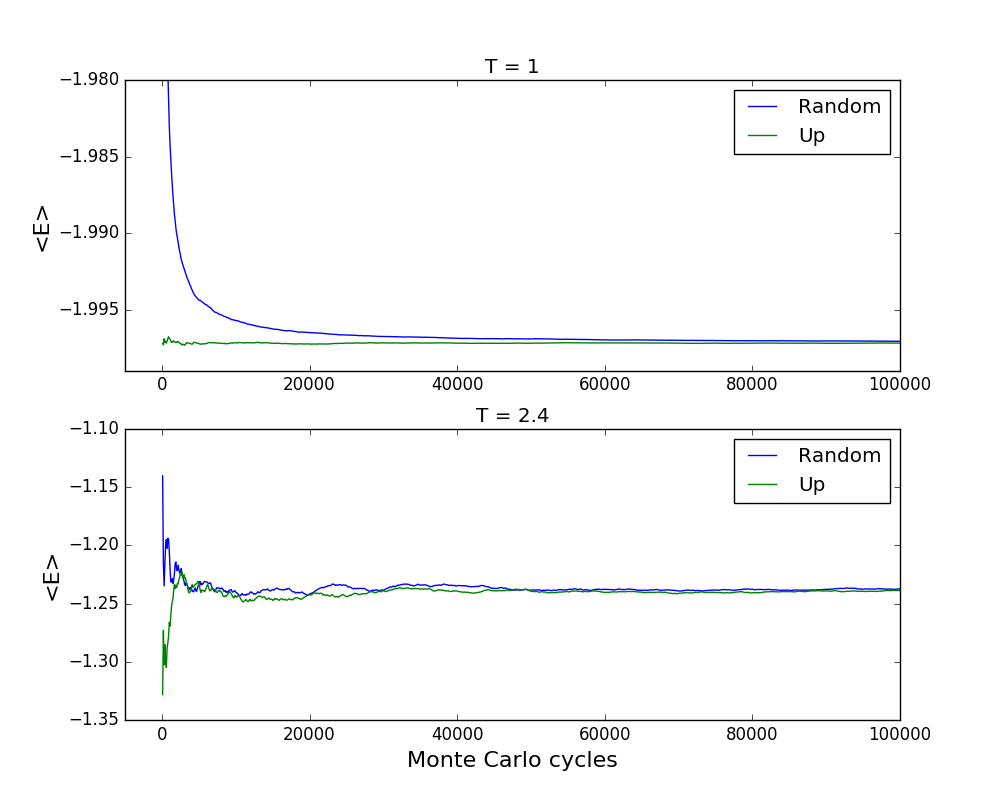
\includegraphics[scale=0.29]{../figures/task_c/energyeig.png}
    \caption{Energy expectation values}
  \end{subfigure}
  \begin{subfigure}{0.49\textwidth}
    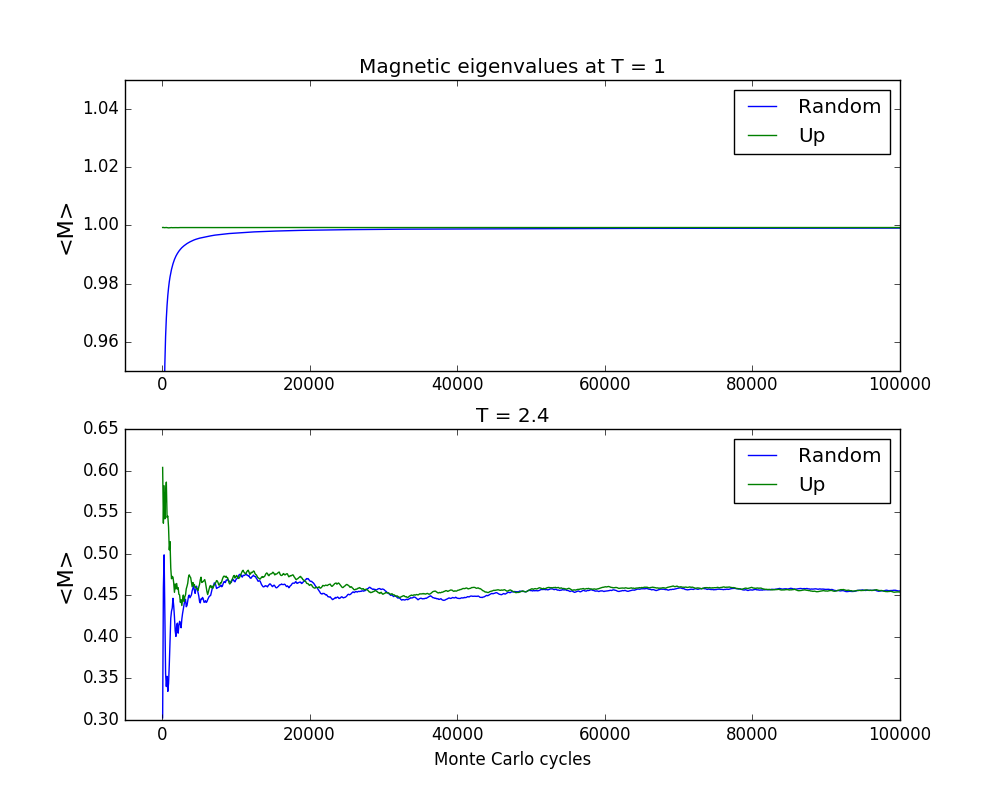
\includegraphics[scale=0.29]{../figures/task_c/Mageig.png}
    \caption{Magnetization expectation values}
  \end{subfigure}
  \caption{Expectation values $E$ as a function of Monte Carlo cycles, for temperatures $T=1.0$ and $T=2.4$, as well as ordered and random initial spin configuration. Lattice size set to $L=20$.}
  \label{fig:impala}
\end{figure}
\begin{figure}[H]
  \centering
  \begin{subfigure}{0.49\textwidth}
    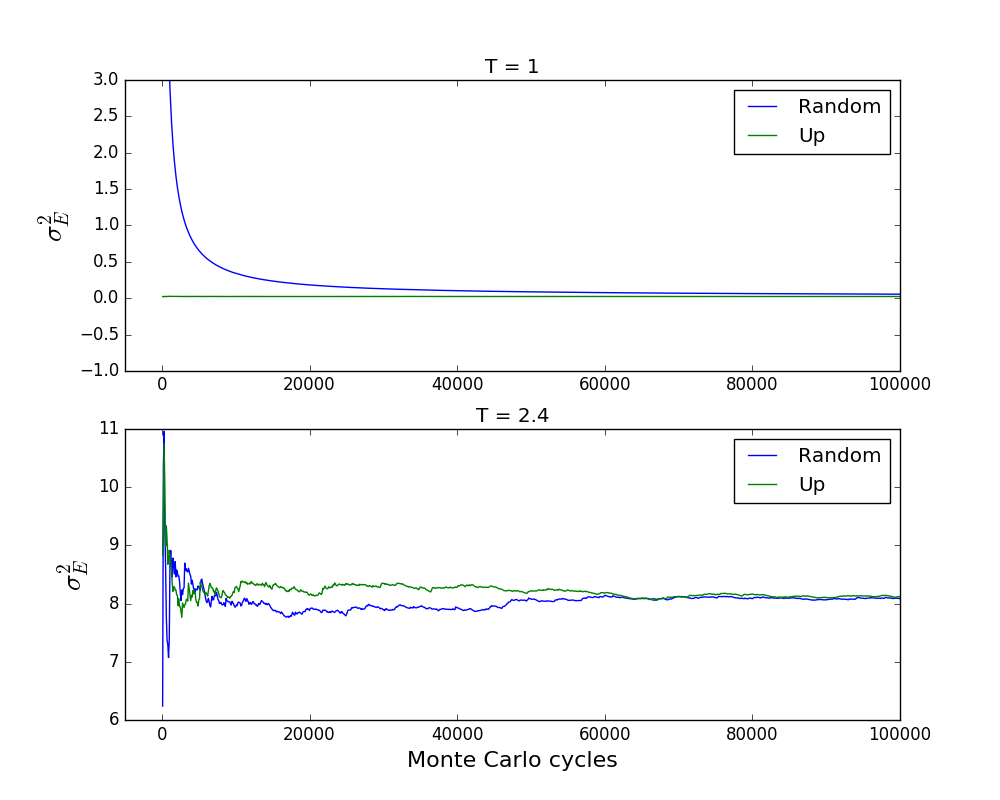
\includegraphics[scale=0.29]{../figures/task_c/sigmaE.png}
    \caption{Specific heat}
  \end{subfigure}
  \begin{subfigure}{0.49\textwidth}
    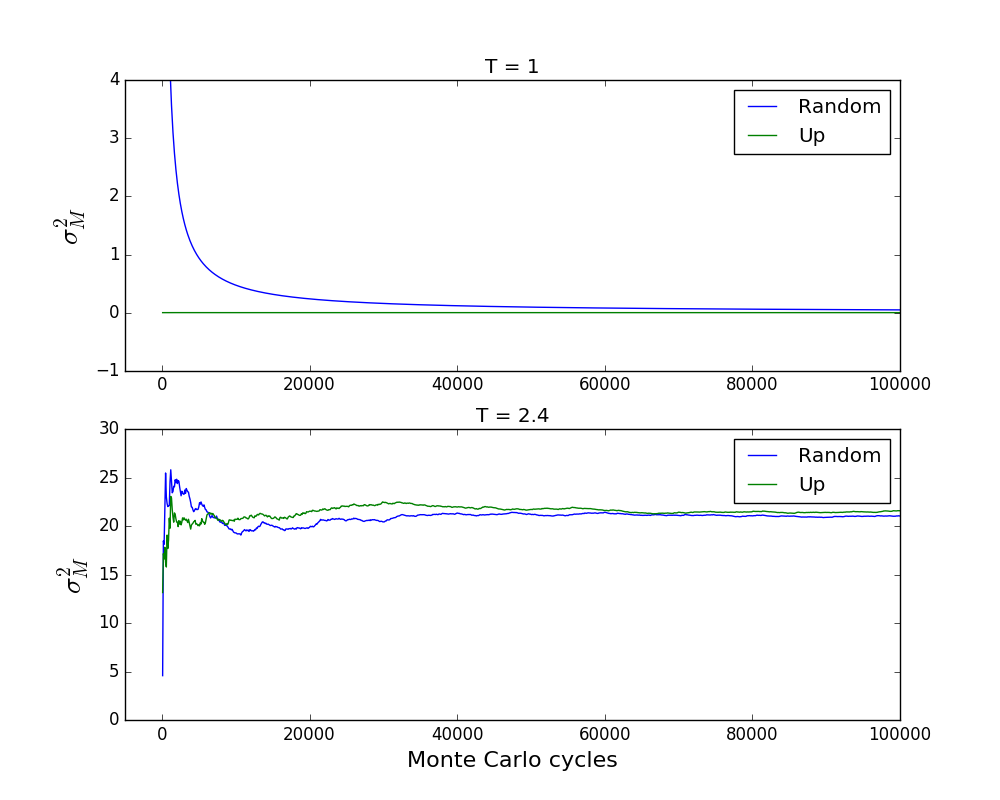
\includegraphics[scale=0.29]{../figures/task_c/sigmaM.png}
    \caption{Magnetic susceptibility}
  \end{subfigure}
  \caption{Expectation values of $\mathcal{M}$as a function of Monte Carlo cycles, for temperatures $T=1.0$ and $T=2.4$, as well as ordered and random initial spin configuration. Lattice size set to $L=20$.}
  \label{fig:imploder}
\end{figure}
In figure \ref{fig:accept}, we see how the number of accepted spin configurations evolve as a function of Monte Carlo cycles for both temperatures.
\begin{figure}[H]
  \centering
  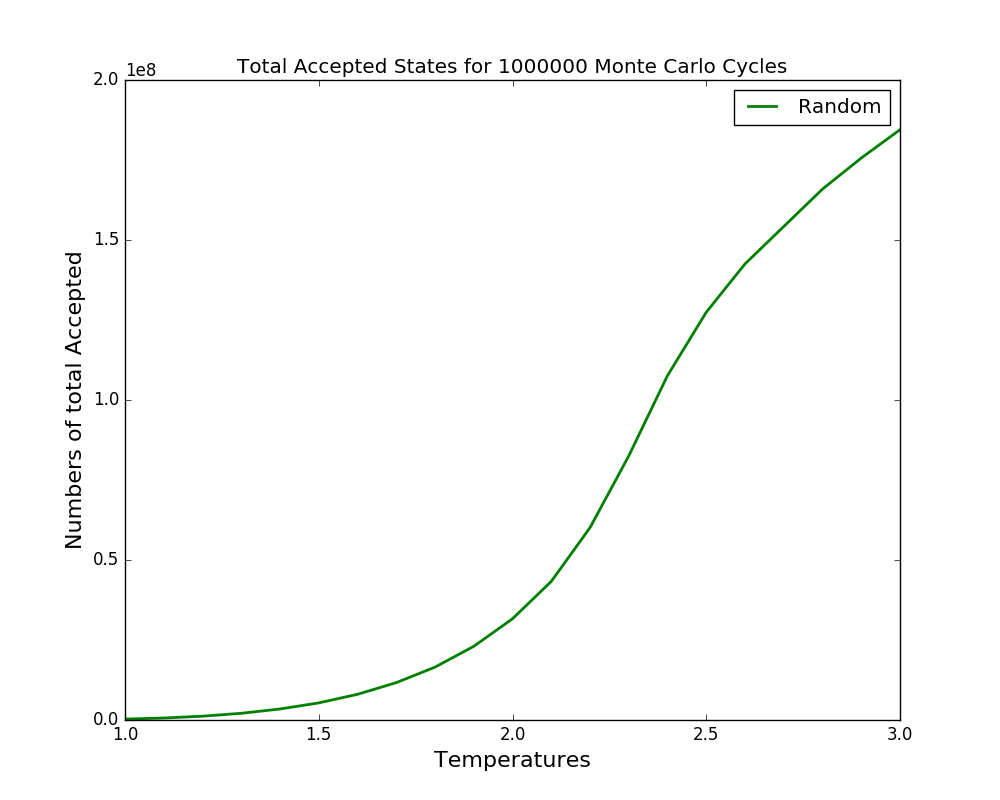
\includegraphics[scale=0.5]{../figures/task_c/accepted.png}
  \caption{Accepted spin configurations plotted as a function of Monte Carlo cycles for $T = 1.0$ and $T=2.4$ for random and ordered initial spin configuration. Lattice size set to $L=20$.}
  \label{fig:accept}
\end{figure}

\subsection{Analyzing the probability distribution}
Shown in figure \ref{fig:historietimen} is the probability $P(E)$ for the system with $L=20$ at temperatures $T=1.0$ and $T=2.4$. In table \ref{tab:noo} the variance of the mean energy $\langle E\rangle$ is shown.
\begin{figure}[H]
  \centering
  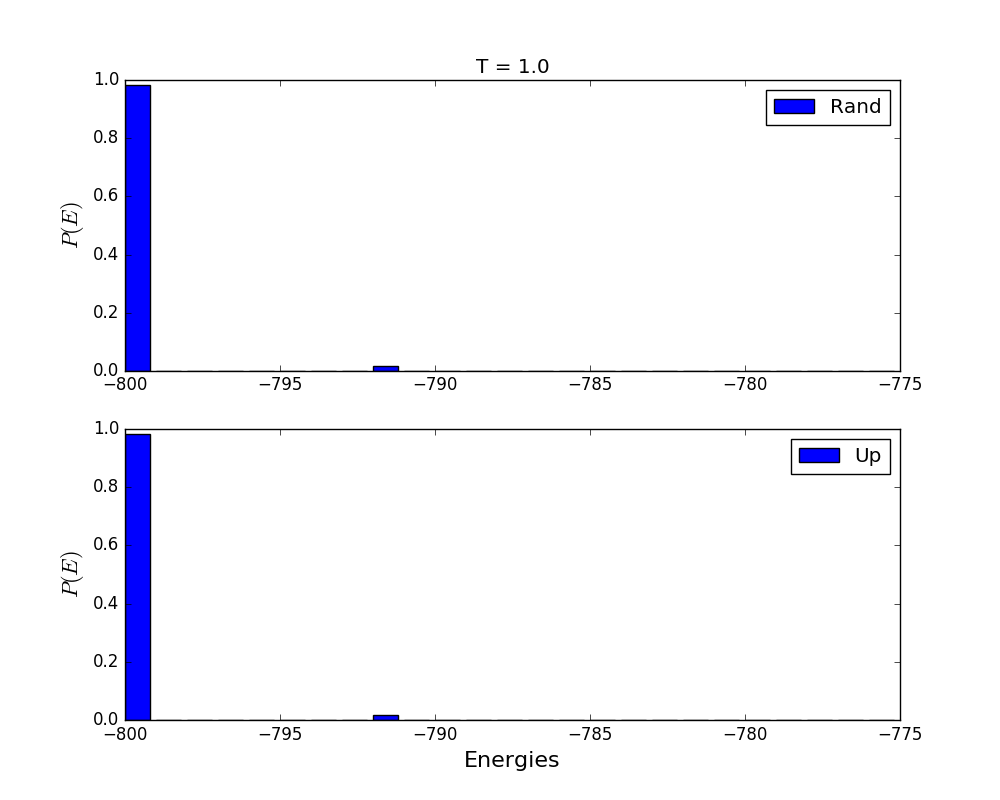
\includegraphics[scale=0.5]{../figures/task_d/hist1.png}
  \caption{Probability $P(E)$ as function of the energy, plotted for $T=1.0$ and $T=2.4$. Lattice size set to $L=20$, and spin configuration ``up''.}
  \label{fig:historietimen}
\end{figure}

\begin{table}[H]
  \centering
  \label{tab:noo}
  \caption{Comparison between the variance of the energy at temperatures $T=1.0$ and $T=2.4$. \textit{results} are computed with applying \texttt{numpy.var()} on the energies saved after the system stabilizes, while \textit{computed} is the variance computed throughout the simulation, and written at the last Monte Carlo cycle, which was set to $10^6$. Units per spin.}
  \begin{tabular}{c|c|c}
    & $\sigma_E^2(T=1.0)$ & $\sigma_E^2(T=2.4)$\\\hline
    results & 0.00292 & 4.11097\\
    computed & 0.02347& 8.09108\\
  \end{tabular}
\end{table}

\subsection{Numerical studies of phase transitions}
Figure \ref{fig:ee} and \ref{fig:harold} shows the different quantities plotted against different temperatures, with varying lattice sizes $L$.

\begin{figure}[H]
  \centering
  \begin{subfigure}{0.49\textwidth}
    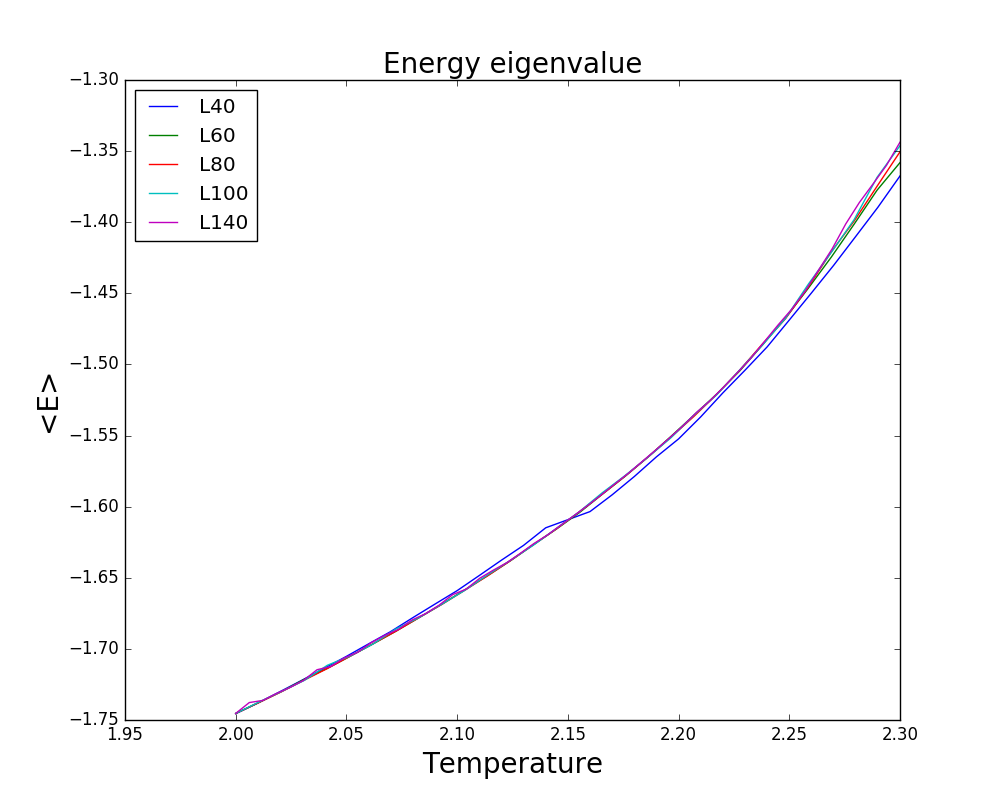
\includegraphics[scale=0.29]{../figures/task_e/energyeig.png}
    \caption{Energy expectation values}
  \end{subfigure}
  \begin{subfigure}{0.49\textwidth}
    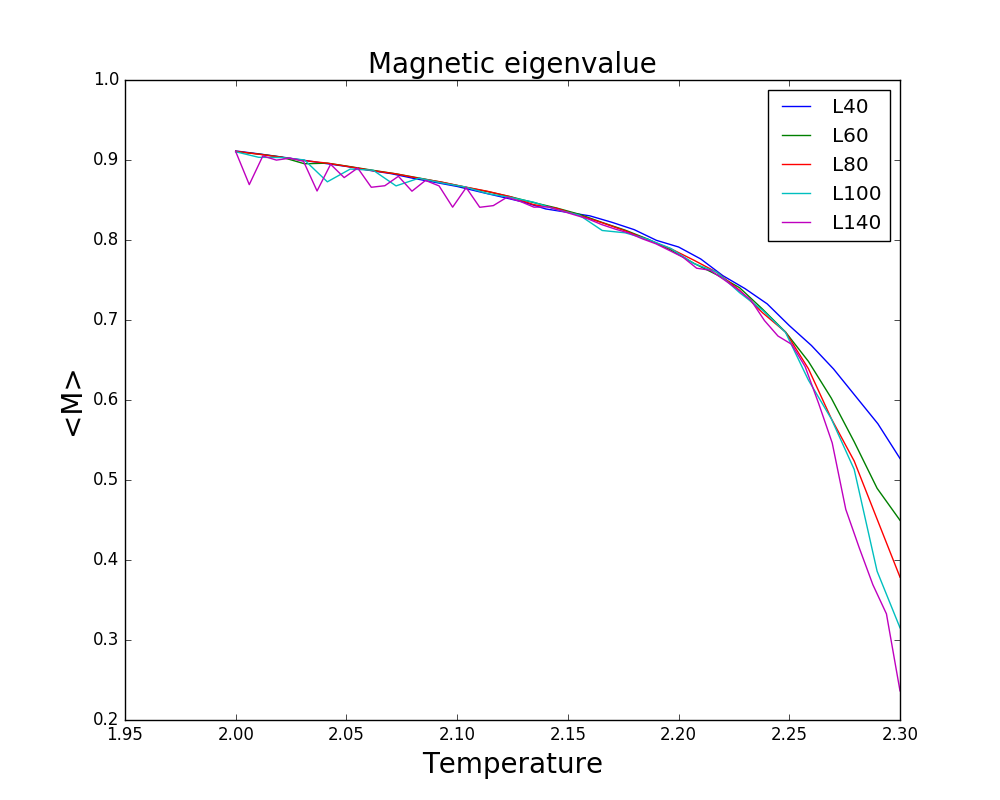
\includegraphics[scale=0.29]{../figures/task_e/Mageig.png}
    \caption{Magnetization expectation values}
  \end{subfigure}
  \caption{Expectation values for $E$ and $|\mathcal{M}|$ as function of temperature for different lattice sizes $L$.}
  \label{fig:ee}
\end{figure}

\begin{figure}[H]
  \centering
  \begin{subfigure}{0.49\textwidth}
    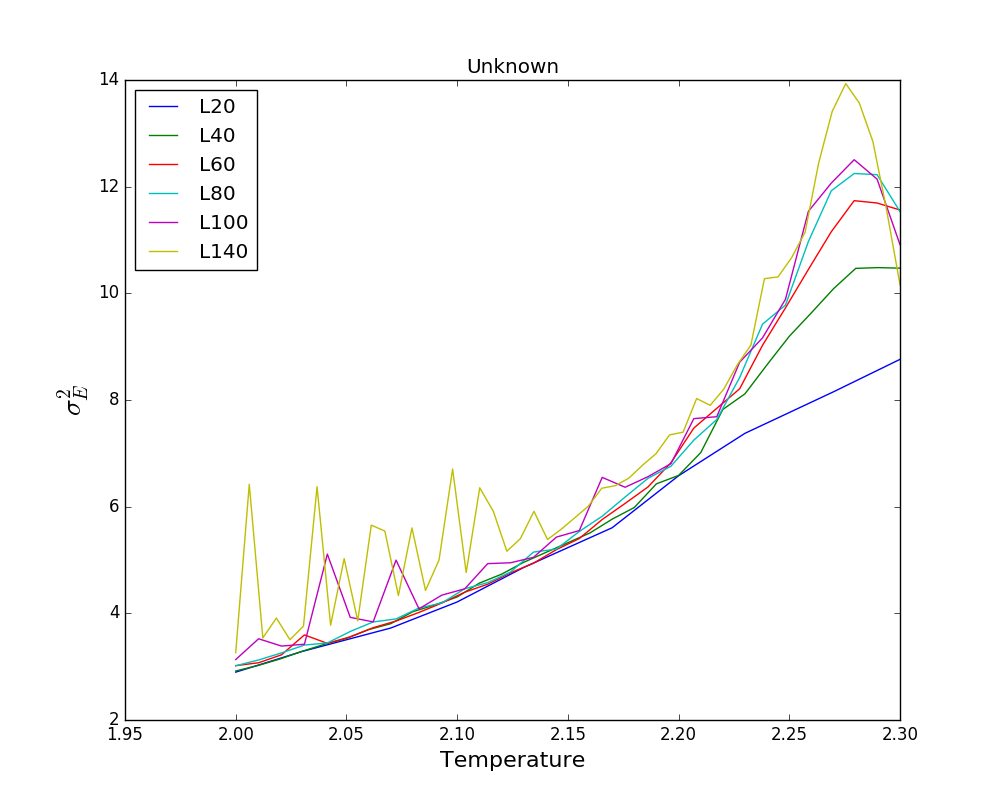
\includegraphics[scale=0.29]{../figures/task_e/sigmaE.png}
    \caption{Specific heat}
  \end{subfigure}
  \begin{subfigure}{0.49\textwidth}
    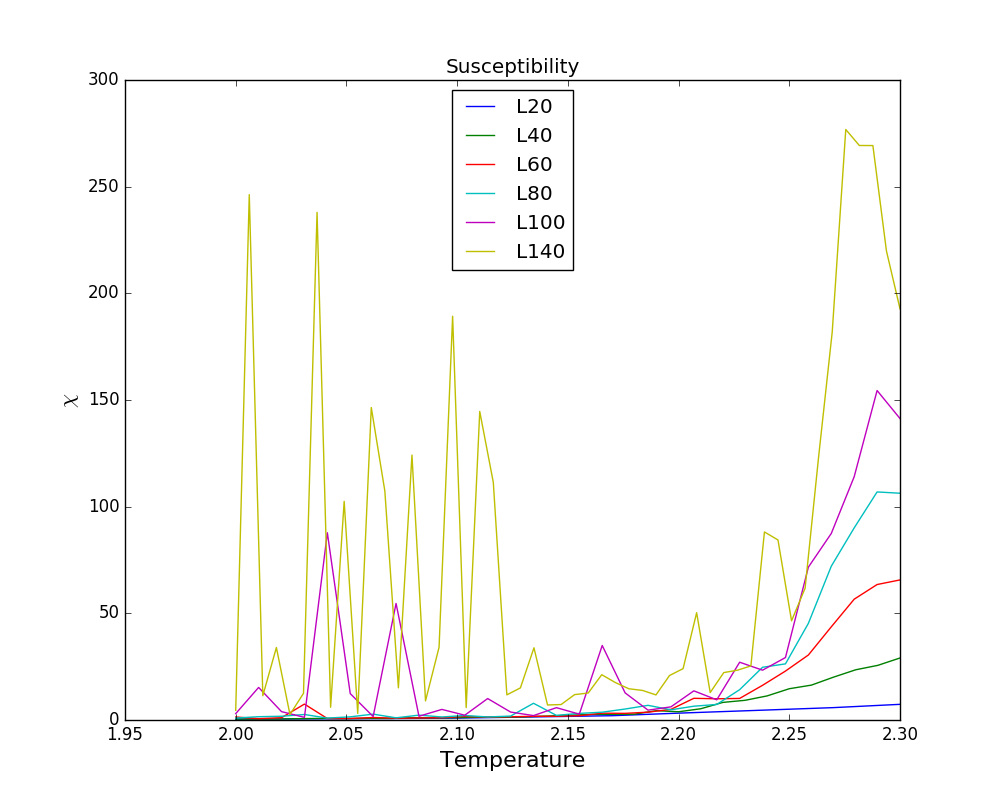
\includegraphics[scale=0.29]{../figures/task_e/accepted.png}
    \caption{Magnetic susceptibility}
  \end{subfigure}
  \caption{Plot of the specific heat and magnetic susceptibility as a function of temperature for different lattice sizes $L$.}
  \label{fig:harold}
\end{figure}

\section{Discussion}
\subsection{Numerical solution of the $2\times2$ model}
From table \ref{tab:meow}, we see that the analytical and numerical values correlate pretty well as the number of Monte Carlo cycles increase. For $\langle E\rangle$ and $\langle|\mathcal{M}|\rangle$, they match at even fairly low number of Monte Carlo cycles. The specific heat and magnetic susceptibility however require a lot higher number of iterations in order to get decent accuracy.\\\\
In order to achieve a good agreement for all quantities, we need somewhere between $10\,000$ and $100\,000$ Monte Carlo cycles, but probably closer to the latter.

\subsection{Thermalisation}
Looking at figures \ref{fig:impala} and \ref{fig:imploder}, we see that for temperature $T = 1.0$, the system stabilizes almost immidiately (less than $10\,000$ cycles) for an ordered initial state, while the random start does not really stabilize before somewhere around $60-80\,000$ cycles. If we look back at table \ref{tab:spins}, we recall that for the simple $2\times2$, the ordered states had the lowest energy. This is true for a larger lattice as well, which explains why the ordered initial configuration is stable from the almost from the start.\\\\
For the higher temperature $T=2.4$, we note that this is higher than the Onsager critical temperature for the system, $T_c = 2.269$, where above that the system enters a phase with no magnetization. For this temperature, the random starting point seems to be slightly closer to the thermal equilibrium, but both of them needs a similar number of Monte Carlo cycles in order to stabilize. In both temperature cases, the systems seem to stabilize at around $60-80\,000$ Monte Carlo cycles.\\\\
Figure \ref{fig:accept} shows the acceptance as a function of Monte Carlo cycles. We note that there is a linear growth as function of cycles, which is not surprising. This applies to both temperatures, but we see that the acceptance increases faster for $T=2.4$ than for $T=1.0$. This shows that as the temperature increases, the likelihood of a configuration getting accepted increases. Looking at the Metropolis algorithm \ref{alg:metropolis}, we see that what decides if we accept it or not is if a randomly drawn number is less than or equal to $e^{-\beta\Delta E}$. Seeing as $\beta \propto 1/T$, increasing $T$ should make the acceptance increase.\\\\
To see this relation more clearly, we could make a plot of the acceptance as function of many different temperatures $T$, but sadly that has yet to be done.

\subsection{Analyzing the probability distribution}
In figure \ref{fig:historietimen}, we see some interesting results for $T=1.0$. As we previously discussed, the equilibrium seems to be an ordered spin configuration with all spins pointing in one direction, which is clearly shown to be the case in this plot. The other \textit{peak} at an energy difference $\Delta E = 8$ away also fits with what we saw earlier in table \ref{tab:spins}.\\\\
For $T=2.4$, we get a probability distribution that closely resembles a normal distribution. \\\\
Table 3 shows the variance in energy $\sigma_E^2$, however the values computed from the histogram in figure \ref{fig:historietimen} are most likely computed and/or scaled wrong.\\\\
There also seems to be something off with the normalization of the $T=1.0$ plot.
\subsection{Numerical studies of phase transitions}
From the figures in the section, we see that the specific heat and magnetic susceptibility peaks at some value for the different lattice sizes. Finding these peaks, and using the equations discussed earlier, we get a critical temperatures
\begin{table}[H]
\centering
\caption{$T_C$ for $C_v$ and $\chi$ as a function of L}
\begin{tabular}{c|c|c}
L & $C_v$ & $\chi$ \\ \hline
40 & 2.28 & 2.3 \\
60 & 2.2793 & 2.3 \\
80 & 2.2793 & 2.2897 \\
100 & 2.2793 & 2.2897 \\
140 & 2.2755 & 2.2755 \\
\end{tabular}
\label{tab:e}
\end{table}
Comparing this to the critical temperature from Onsager \cite{cite:lars_onsager} ($T_C = 2.269$), we see that our simulations yield quite nice results.\\\\
The calculations for the final task (with different $L$ values), was run on 30 cores at the same time, and found to be significantly faster than what it would have been if running on one core.

%\href{{http://journals.aps.org/pr/abstract/10.1103/PhysRev.65.117}
\bibliography{references}{}
\bibliographystyle{plain}

\end{document}
